\section{Learning and predicting single-cell responses with \textsc{CellOT}}
% TODO: minor: connect flow

% Small molecule drugs can have profound effects on the cellular phenotype by, for instance, altering signaling cascades.
% Most of these effects depend on the context in which the perturbation occurs.
% Given the heterogeneity among single cells in cell populations and tissues, predicting cellular responses requires understanding the rules by which context shapes genome activity and its response to drugs.
% High-dimensional single-cell data measured via single-cell genomics or multiplexed imaging technologies can provide this contextual information but only return  unpaired or unaligned observations of cell populations.
% Here, \textsc{CellOT} allows us to utilize such unpaired data and enables learning cell state transitions upon perturbation.

We denote the unperturbed control population by $\mu$ consisting of $n$ cells $x_i$ for $i = 1, \dots, n$.
Upon perturbation $k$, the multivariate state of each cell $x_i$ of the unperturbed population changes, which we observe as the perturbed population $\nu$ (Fig \ref{fig:cellot-overview}a).
To understand the mode of action and effect of perturbations, we seek to learn the transition and alignment between populations $\mu$ and $\nu$ via parameterizing a map $T$ (see \textbf{Fig \ref{fig:cellot-overview}a-b}), which explains the transition of each cell from the unperturbed cell population $\mu$ into their perturbed state $\nu$ upon treatment $k$.
Despite originating from  different observations, map $T$ determines for each cell $x_i$ the most likely corresponding cell $T(x_i)$ in the perturbed population (\textbf{Fig \ref{fig:cellot-overview}c}).
Finding this map then not only allows us to model single-cell trajectories upon perturbation but also to predict the perturbed state of previously unseen control cells.
As a result, we can forecast the outcome of a perturbation $k$  by applying the learned map $T$ to a new unperturbed population $\rho^\prime_c$ (\textbf{Fig \ref{fig:cellot-overview}d}).

The optimal map $T$ aligning the control and perturbed population, which we seek to find, should best describe the incremental changes in the multivariate profile of each cell after applying a perturbation $k$.
Using optimal transportation theory \cite{villani2021topics, santambrogio2015optimal} to recover these maps and unveil single-cell reprogramming trajectories has been proposed as a strong modeling hypothesis in the domain of single-cell biology \cite{schiebinger2019optimal, cang2020inferring, demetci2020gromov, huizing2021optimal, lavenant2021towards, zhang2021optimal}.
Optimal transport problems return the alignment between distributions $\mu$ and $\nu$ corresponding to the minimal overall cost between aligned molecular profiles, thus determining the most likely state of each cell upon perturbation (Fig \ref{fig:cellot-overview}c).
$T$ is learned such that its image corresponds to $\nu$ and mass is moved from $\mu$ into $\nu$ according to a principle of minimal effort.
% Utilizing recent advancements in neural optimal transport theory, \textsc{CellOT} considers the dual form of the transport problem and parameterizes a pair of convex potentials with neural networks.
$T$ is recovered as the gradient of one of these potentials.
As directly parameterizing the optimal transport map $T$ \cite{korotin2019wasserstein, yang2018scalable, prasad2020optimal} is unstable \citep[Table 1]{makkuva2020optimal}, we parameterize the convex potentials of the dual optimal transport problem $f$ and $g$ by convex neural networks \cite{amos2017input} and recover the optimal map $T$ using the gradient of a convex function $g_k$, i.e., $\nabla g_k$ \cite{makkuva2020optimal}.

To put \textsc{CellOT}'s performance in perspective, we benchmark it against current state-of-the-art autoencoder-based methods cite{lotfollahi2019scgen, Lopez2018scvi},
which attempt to add perturbation effects through the manipulation of a learned latent representation (review in Supplementary Section \ref{supp:related_work}).
To further test the hypothesis of the optimal transport modeling prior, we compare the learned OT map $\nabla g_k$ for each perturbation $k$ with naive non-OT-based alignments.


\begin{figure}
  \begin{center}
  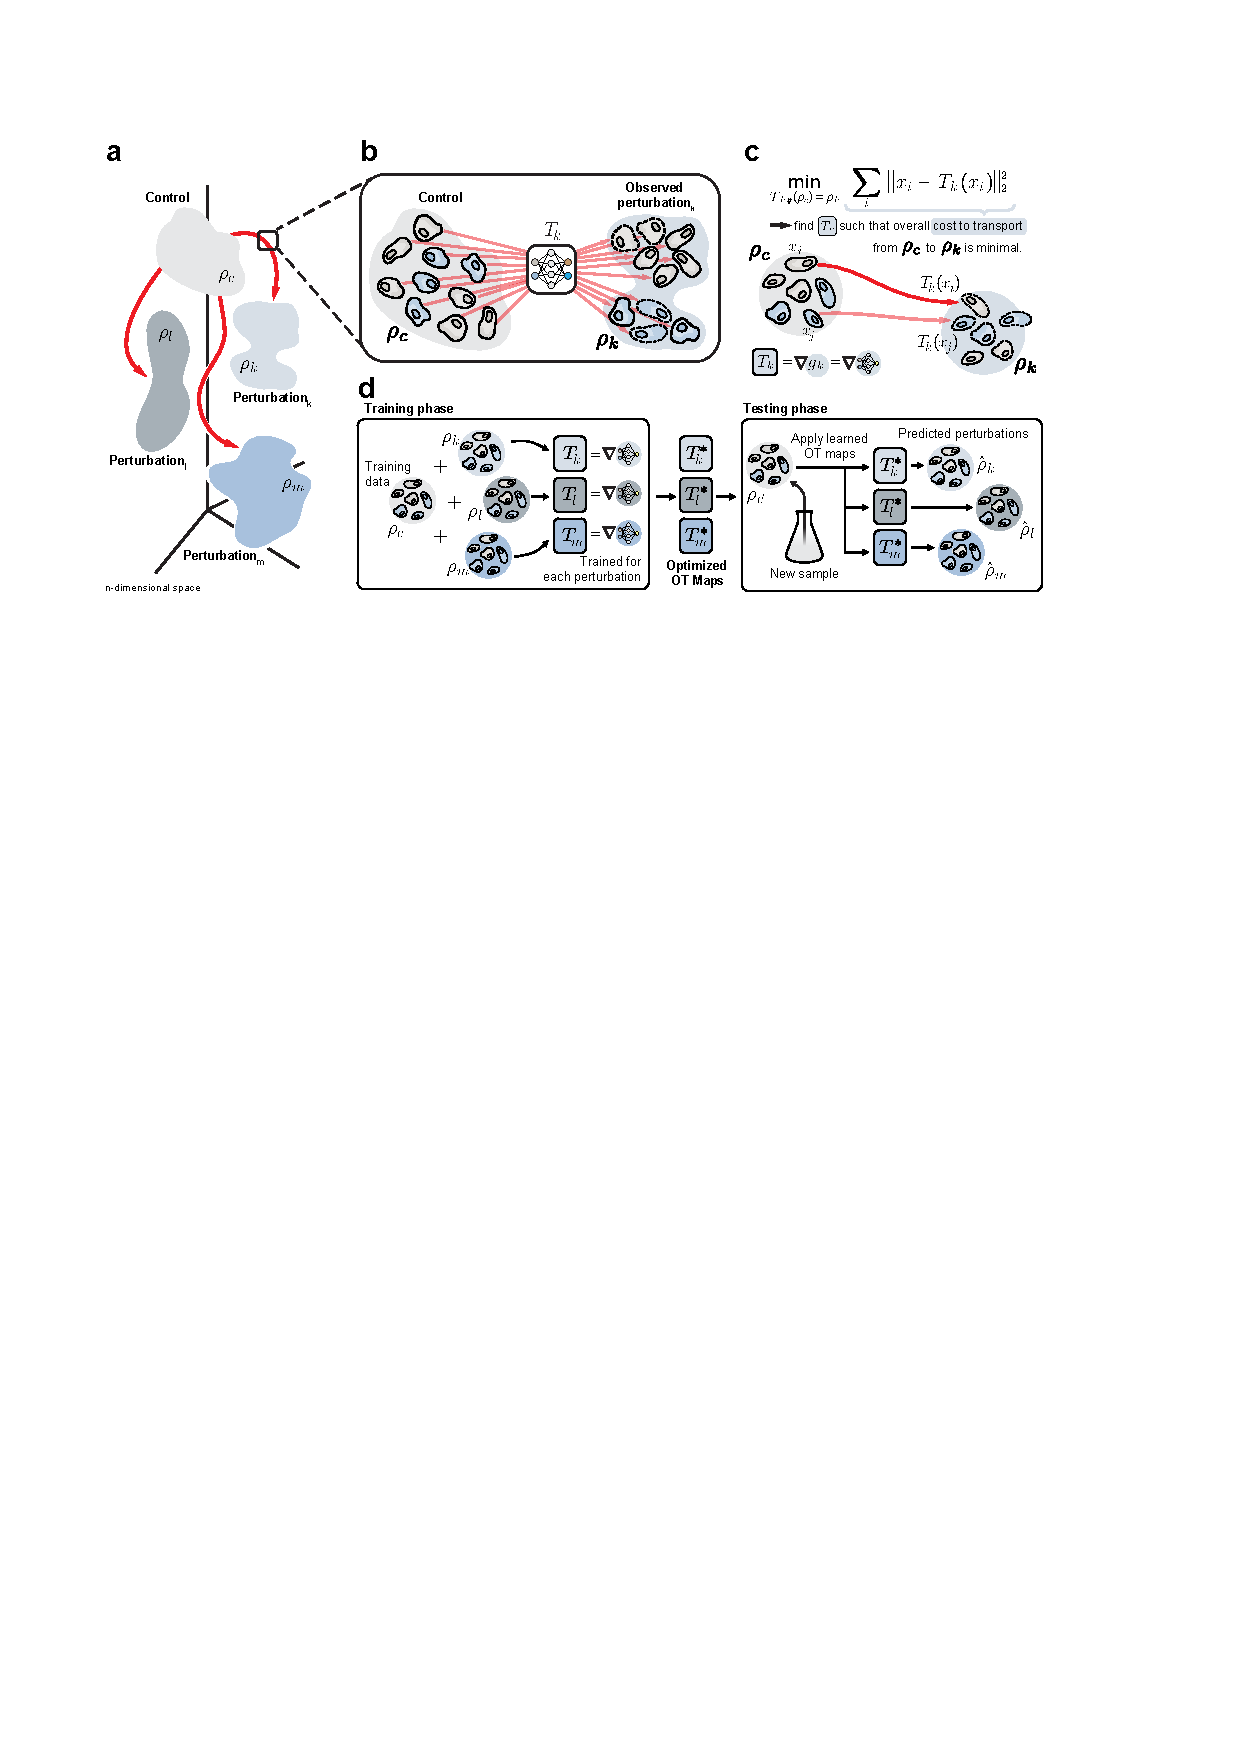
\includegraphics[width=0.95\textwidth]{figures/cellot-methods/Bunne_Main_Fig1.pdf}
  \end{center}
  \caption{Overview of the \textsc{CellOT} Model. \textbf{a)}~Distributions of single cells were measured in either an untreated control state ($\rho_c$) or in one of several perturbed states ($\rho_k, \rho_l, \rho_m,  \ldots$). These distributions lie in a high-dimensional space of profiled features. \textbf{b)}~For a perturbation $k$, we aim to model it with a function $T_k$ that maps untreated cells in $\rho_c$ to their treated counterparts in $\rho_k$. \textbf{c)}~Lacking paired measurements, we assume that the perturbation transforms $\rho_c$ into $\rho_k$ under a principle of minimal effort. In particular, we learn $T_k$ using optimal transport theory to directly estimate this distributional mapping as the gradient of the optimal transport dual potential $\nabla g_\theta$.
    \textbf{d)}~OT maps are learned for all perturbations independently. Because these maps are fully parameterized, \textsc{CellOT} can be trained, for example, on a set of initially provided samples to then make predictions on untreated cells originating from new, previously unseen samples.}
  \label{fig:cellot-overview}
\end{figure}

\subsection{Evaluation strategies}
% TODO: check wording 
Since we lack access to the ground truth set of control and treatment observations on the single-cell level,
we analyze the effectiveness of \textsc{CellOT} using evaluations that operate on the level of the distribution of real and predicted perturbation states.
Three metrics are considered, i.e., MMD, $\ell_2$ feature means, and the average correlation of the feature means.

$\ell_2$ feature means refers to the $\ell_2$-distance between means of the observed and predicted distributions. Similarly, $r$ feature means refers to the correlation of the means of the observed and predicted distributions.
However, metrics based only on feature means can be insensitive in settings where heterogeneity is not captured. Consider, for example, a target distribution with multiple modes. These metrics will favorably evaluate a uni-modal predicted distribution that simply models the mean of this multi-modal distribution. To this end, we include a distributional distance sensitive to this type of behavior by measuring differences in the properties of higher moments, i.e., the maximum mean discrepancy.
% Let $r_c$ be a set of observed untreated cells, $r_k$ be a set of observed cells treated with perturbation $k$, and $\hat{r}_k$ be the set of predictions made on $r_c$. The drug signature of perturbation is defined as:
% \begin{equation*}
%     DS(r_k, r_c) = \frac{1}{|r_k|}\sum_{x_i \in r_k}{x_i} - \frac{1}{|r_c|}\sum_{y_i \in r_c}{y_i}
% \end{equation*}
% We report the $\ell_2$ distance between the observed signature $DS(r_k, r_c)$ and the predicted signature $DS(\hat{r}_k, r_c)$, which is a function of the difference in the means between the observed and predicted distributions.

MMD refers to the kernel maximum mean discrepancy \citep{gretton2012kernel}, a metric to measure distances between distributions.
Given two random variables x and y with distributions p and q, and a kernel function $\phi$, \citet{gretton2012kernel} define the squared MMD as
\begin{equation*}
    \text{MMD}(p, q; \phi) = \mathbb{E}_{x,x^\prime}[\phi(x, x^\prime)] + \mathbb{E}_{y,y^\prime}[\phi(y, y^\prime)] - 2\mathbb{E}_{x,y}[\phi(x, y)].
\end{equation*}
We report an unbiased estimate of $\text{MMD}(r_k, \hat{r}_k)$ where the expectations are evaluated by averages over the cells in each set. The RBF kernel is employed, and as is usually done, reports the MMD as an average over several length scales, i.e., \texttt{np.logspace(1, -3)}.

